\documentclass[a4paper, 14pt]{extarticle}

% Поля
%--------------------------------------
\usepackage{geometry}
\geometry{a4paper,tmargin=2cm,bmargin=2cm,lmargin=3cm,rmargin=1cm}
%--------------------------------------


%Russian-specific packages
%--------------------------------------
\usepackage[T2A]{fontenc}
\usepackage[utf8]{inputenc} 
\usepackage[english, main=russian]{babel}
%--------------------------------------

\usepackage{textcomp}

% Красная строка
%--------------------------------------
\usepackage{indentfirst}               
%--------------------------------------             


%Graphics
%--------------------------------------
\usepackage{graphicx}
\graphicspath{ {./images/} }
\usepackage{wrapfig}
%--------------------------------------

\usepackage{listings}
\usepackage{color}
\definecolor{dkgreen}{rgb}{0,0.6,0}
\definecolor{gray}{rgb}{0.5,0.5,0.5}
\definecolor{mauve}{rgb}{0.58,0,0.82}
\lstset{frame=tb,
  language=Java,
  aboveskip=3mm,
  belowskip=3mm,
  showstringspaces=false,
  columns=flexible,
  basicstyle={\small\ttfamily},
  numbers=none,
  numberstyle=\tiny\color{gray},
  keywordstyle=\color{blue},
  commentstyle=\color{dkgreen},
  stringstyle=\color{mauve},
  breaklines=true,
  breakatwhitespace=true,
  tabsize=3
}

% Полуторный интервал
%--------------------------------------
\linespread{1.3}                    
%--------------------------------------

%Выравнивание и переносы
%--------------------------------------
% Избавляемся от переполнений
\sloppy
% Запрещаем разрыв страницы после первой строки абзаца
\clubpenalty=10000
% Запрещаем разрыв страницы после последней строки абзаца
\widowpenalty=10000
%--------------------------------------

%Списки
\usepackage{enumitem}

%Подписи
\usepackage{caption} 

%Гиперссылки
\usepackage{hyperref}

\hypersetup {
	unicode=true
}

%Рисунки
%--------------------------------------
\DeclareCaptionLabelSeparator*{emdash}{~--- }
\captionsetup[figure]{labelsep=emdash,font=onehalfspacing,position=bottom}
%--------------------------------------

\usepackage{tempora}

%Листинги
%--------------------------------------
\usepackage{listings}
\lstset{
  basicstyle=\ttfamily\footnotesize, 
  %basicstyle=\footnotesize\AnkaCoder,        % the size of the fonts that are used for the code
  breakatwhitespace=false,         % sets if automatic breaks shoulbd only happen at whitespace
  breaklines=true,                 % sets automatic line breaking
  captionpos=t,                    % sets the caption-position to bottom
  inputencoding=utf8,
  frame=single,                    % adds a frame around the code
  keepspaces=true,                 % keeps spaces in text, useful for keeping indentation of code (possibly needs columns=flexible)
  keywordstyle=\bf,       % keyword style
  numbers=left,                    % where to put the line-numbers; possible values are (none, left, right)
  numbersep=5pt,                   % how far the line-numbers are from the code
  xleftmargin=25pt,
  xrightmargin=25pt,
  showspaces=false,                % show spaces everywhere adding particular underscores; it overrides 'showstringspaces'
  showstringspaces=false,          % underline spaces within strings only
  showtabs=false,                  % show tabs within strings adding particular underscores
  stepnumber=1,                    % the step between two line-numbers. If it's 1, each line will be numbered
  tabsize=2,                       % sets default tabsize to 8 spaces
  title=\lstname                   % show the filename of files included with \lstinputlisting; also try caption instead of title
}
%--------------------------------------

%%% Математические пакеты %%%
%--------------------------------------
\usepackage{amsthm,amsfonts,amsmath,amssymb,amscd}  % Математические дополнения от AMS
\usepackage{mathtools}                              % Добавляет окружение multlined
\usepackage[perpage]{footmisc}
%--------------------------------------

%--------------------------------------
%			НАЧАЛО ДОКУМЕНТА
%--------------------------------------

\begin{document}

%--------------------------------------
%			ТИТУЛЬНЫЙ ЛИСТ
%--------------------------------------
\begin{titlepage}
\thispagestyle{empty}
\newpage


%Шапка титульного листа
%--------------------------------------
\vspace*{-60pt}
\hspace{-65pt}
\begin{minipage}{0.3\textwidth}
\hspace*{-20pt}\centering

\includegraphics[width=\textwidth]{emblem}
\end{minipage}
\begin{minipage}{0.67\textwidth}\small \textbf{
\vspace*{-0.7ex}
\hspace*{-6pt}\centerline{Министерство науки и высшего образования Российской Федерации}
\vspace*{-0.7ex}
\centerline{Федеральное государственное бюджетное образовательное учреждение }
\vspace*{-0.7ex}
\centerline{высшего образования}
\vspace*{-0.7ex}
\centerline{<<Московский государственный технический университет}
\vspace*{-0.7ex}
\centerline{имени Н.Э. Баумана}
\vspace*{-0.7ex}
\centerline{(национальный исследовательский университет)>>}
\vspace*{-0.7ex}
\centerline{(МГТУ им. Н.Э. Баумана)}}
\end{minipage}
%--------------------------------------

%Полосы
%--------------------------------------
\vspace{-25pt}
\hspace{-35pt}\rule{\textwidth}{2.3pt}

\vspace*{-20.3pt}
\hspace{-35pt}\rule{\textwidth}{0.4pt}
%--------------------------------------

\vspace{1.5ex}
\hspace{-35pt} \noindent \small ФАКУЛЬТЕТ\hspace{80pt} <<Информатика и системы управления>>

\vspace*{-16pt}
\hspace{47pt}\rule{0.83\textwidth}{0.4pt}

\vspace{0.5ex}
\hspace{-35pt} \noindent \small КАФЕДРА\hspace{85pt} <<Теоретическая информатика и компьютерные технологии>>

\vspace*{-16pt}
\hspace{30pt}\rule{0.866\textwidth}{0.4pt}
  
\vspace{11em}

\begin{center}
\Large {\bf Лабораторная работа № 0} \\ 
\large {\bf по курсу <<Языки и методы программирования>>} \\
\large <<Приобретение опыта работы с VDS-сервером под управлением ОС Linux>> 
\end{center}\normalsize

\vspace{8em}


\begin{flushright}
  {Студент группы ИУ9-22Б Лавров Р. Д. \hspace*{15pt}\\ 
  \vspace{2ex}
  Преподаватель Посевин Д. П.\hspace*{15pt}}
\end{flushright}

\bigskip

\vfill
 

\begin{center}
\textsl{Москва 2025}
\end{center}
\end{titlepage}
%--------------------------------------
%		КОНЕЦ ТИТУЛЬНОГО ЛИСТА
%--------------------------------------

\renewcommand{\ttdefault}{pcr}

\setlength{\tabcolsep}{3pt}
\newpage
\setcounter{page}{2}

\section{Задание}\label{Sect::task}
\begin{enumerate}[nosep]
\item По инструкции настроить учетную запись на удаленном VDS-сервере.
\item В своей учетной записи настроить окружение для удобного запуска компилятора Java.
\item Запустить любой простейший пример приведенный на лекции 1 или на лабораторной работе 1.
\item Запустить веб-сервер из примера на своем порту. Каждый студент резервирует свой собственный порт. Рекомендуется нумерацию портов использовать по следующему правилу: резервировать номер порта "800n", где n - это порядковый номер студента в Электронном университете, другимим словами, если у студента в Электронном университете порядковй номер 3, то порт веб-сервера данного студента будет 8003.
\item Научиться запускать веб-сервер через утилиту screen.
\item Объединить простейший пример с веб-сервером, т.е. результаты работы программы простейшего прмера выводить через веб-сервер.
\item Запустить работу веб-сервера, выполненного в пункте 6 на своем порту.
\item Как только пункты 1-7 выполнены, выслать строго в телеграм-канал в комментарий к условию данной лабораторной работы: URL-страницы результата работы вашего веб-сервера.
\end{enumerate}

\section{Результаты}\label{Sect::res}

Результат создания учётной записи и настройки окружения

\begin{figure}[!htb]
	\centering
	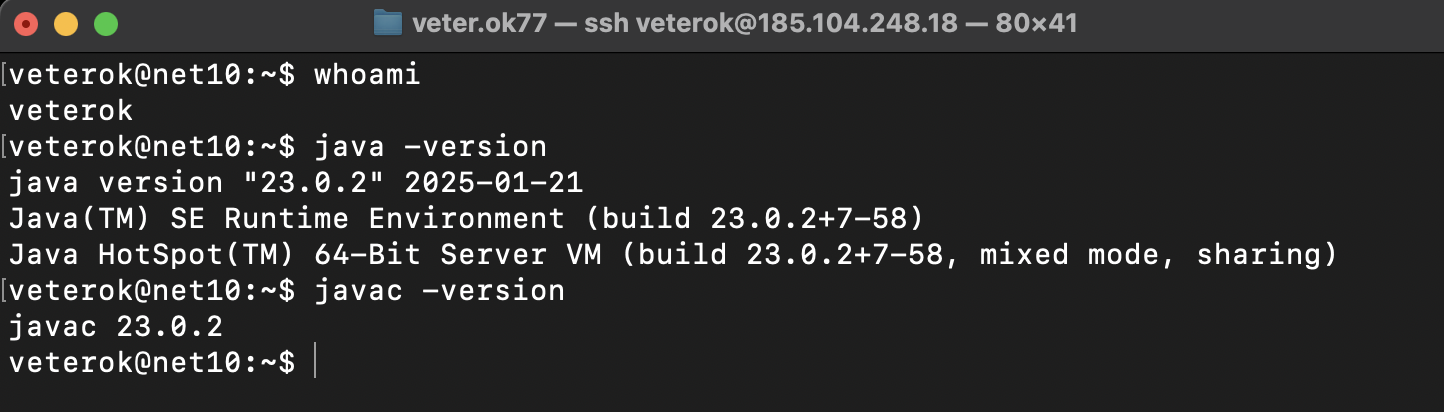
\includegraphics[width=0.8\textwidth]{images/photo1.png}
\caption{Результат}
\label{fig:photo1}
\end{figure}

\newpage

Исходный код простейший программы приведенный на лекцииx~\ref{lst:code1}--~\ref{lst:code2}--~\ref{lst:code3}.

\begin{figure}[!htb]
\begin{lstlisting}[caption={Пример реализации класса}, label={lst:code1}]
public class Dog {
    private String name;
    int age;
    String color;
    int amoutoftails;

    public Dog() {
        System.out.println("The dog was born");
        this.name = "no name"; 
    }

    public Dog(String name) {
        System.out.println("The dog was born"+name);
        this.name = name; 
    }

    public Dog(String name, int age) {
        System.out.println("The dog was born"+name);
        this.name = name; 
        this.age = age; 
    }
    void parse() {}
    void prog() {}
    void getName(String aaa) {
        System.out.println("The dog was born"+aaa);
    }  
    void changeName(String bbb){
        this.name = bbb;
    }

    String getName(){
        return "("+this.name+")";
    }   
}
\end{lstlisting}
\end{figure}

\begin{figure}[!htb]
\begin{lstlisting}[caption={Пример создания экземпляра класса}, label={lst:code2}]
public class Main {
    public static void main(String[] args) {
        Dog a = new Dog("Bobik",40000);
        Dog b = new Dog("Gychka");
        System.out.println("->"+a.getName());
        a.changeName("Innokentiy 2");
        System.out.println("1->"+a.getName());
        a.getName("ssxcxdfvrsvdr");
        System.out.println("age->"+a.age);
        System.out.println("color->"+a.color);
        System.out.println("amoutoftails->"+a.amoutoftails);
    }
}
\end{lstlisting}
\end{figure}

\newpage

\begin{figure}[!htb]
\begin{lstlisting}[caption={Сервер из примера с модификацией}, label={lst:code3}, linewidth=17.6cm, xleftmargin=-0.5cm]
import java.io.BufferedReader;
import java.io.IOException;
import java.io.InputStreamReader;
import java.io.PrintWriter;
import java.net.ServerSocket;
import java.net.Socket;
import java.nio.charset.StandardCharsets;

public class HttpServer {

    public static void main(String[] args) {
        try (ServerSocket serverSocket = new ServerSocket(8294)) {
            System.out.println("Server started!");
            Factorial fact = new Factorial();
            while (true) {
                Socket socket = serverSocket.accept();
                System.out.println("Client connected!");
                BufferedReader input = new BufferedReader(
                    new InputStreamReader(socket.getInputStream(), 
                    StandardCharsets.UTF_8));
                try (PrintWriter output = new PrintWriter(socket.getOutputStream())) {
                    String requestLine = input.readLine();
                    String response = "<p>Incorrect request</p>";
                    output.println("HTTP/1.1 200 OK");
                    System.out.println(requestLine);
                    if (requestLine != null && requestLine.startsWith("GET ")) {
                        String[] parts = requestLine.split(" ");
                        if (parts.length > 1) {
                            String path = parts[1].substring(1);
                            if (isNumber(path) && path != "") {
                                int number = Integer.parseInt(path);
                                response = "<p>fact(" + number + ") = " + fact.count(number) + "</p>";
                            }
                        }
                    }
                    output.println("HTTP/1.1 200 OK");
                    output.println("Content-Type: text/html; charset=utf-8");
                    output.println();
                    output.println(response);
                    output.flush();
                
                    System.out.println("Client disconnected!");
                }
            }
        } catch (IOException ex) {
            ex.printStackTrace();
        }
    }
    private static boolean isNumber(String s) {
        for (int i = 0; i < s.length(); i++) {
            if (!Character.isDigit(s.charAt(i))) {
                return false;
            }
        }
        return true;
    }
}
\end{lstlisting}
\end{figure}

\newpage

\begin{figure}[!htb]
	\centering
	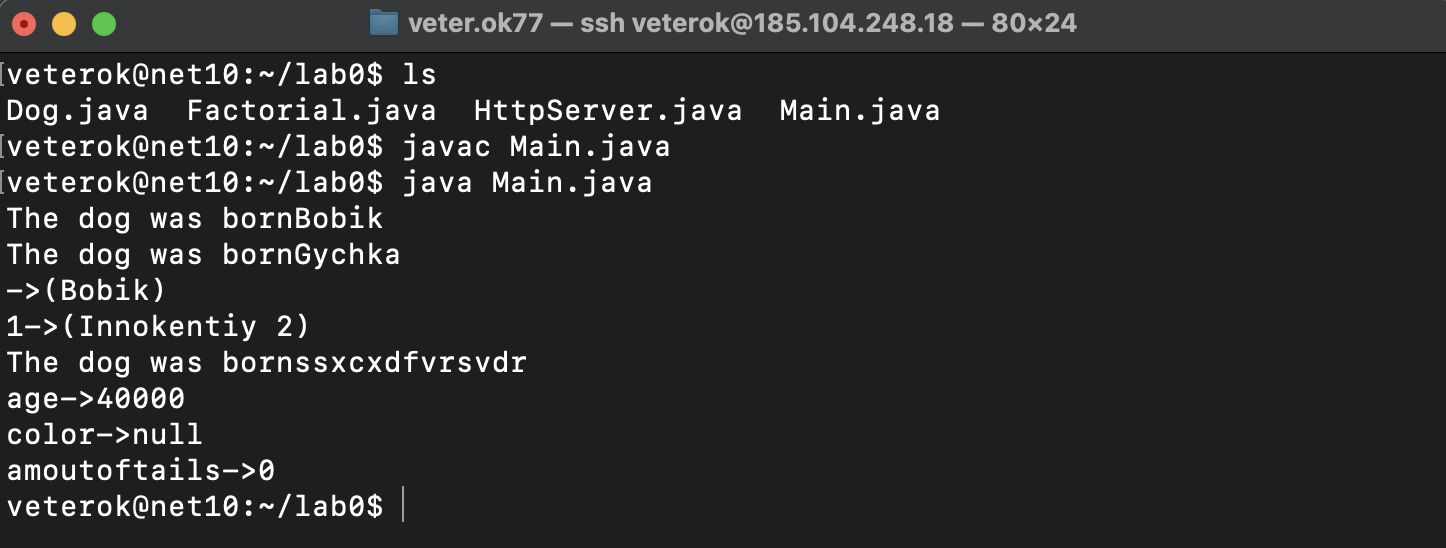
\includegraphics[width=0.8\textwidth]{images/photo2.png}
\caption{Результат запуска Main.java}
\label{fig:photo2}
\end{figure}

\begin{figure}[!htb]
	\centering
	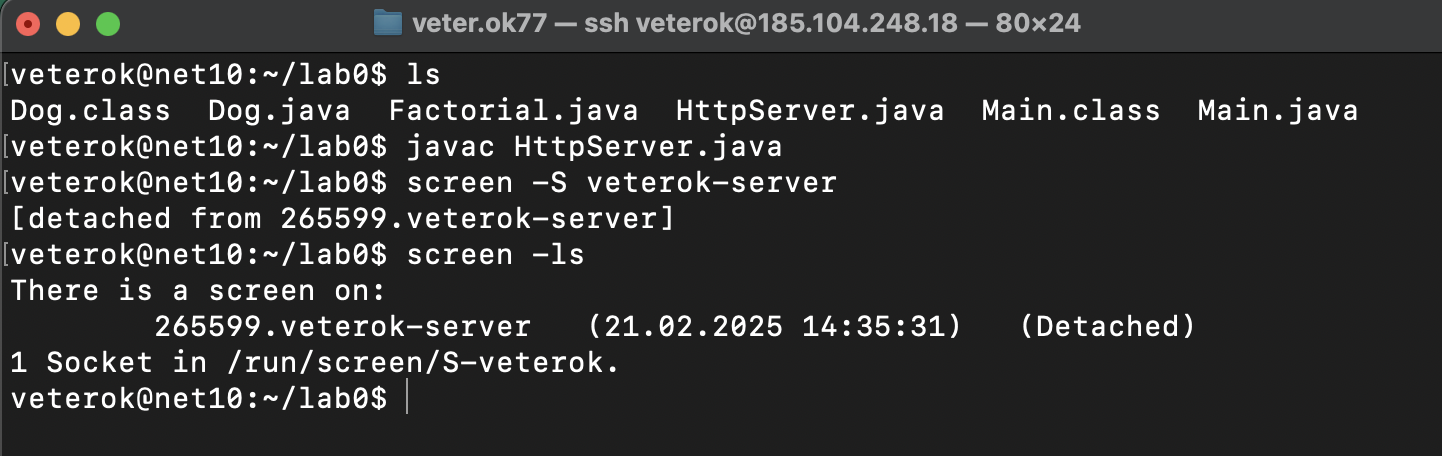
\includegraphics[width=0.8\textwidth]{images/photo3.png}
\caption{Создание screen сессии}
\label{fig:photo2}
\end{figure}

\begin{figure}[!htb]
	\centering
	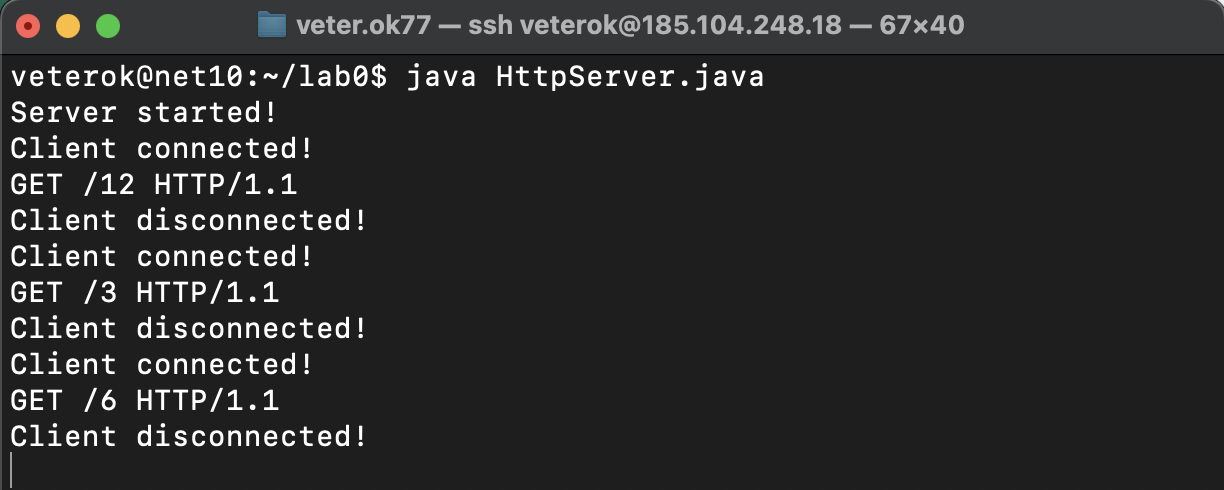
\includegraphics[width=0.8\textwidth]{images/photo4.png}
\caption{Логи работы веб-сервера}
\label{fig:photo2}
\end{figure}

\begin{figure}[!htb]
	\centering
	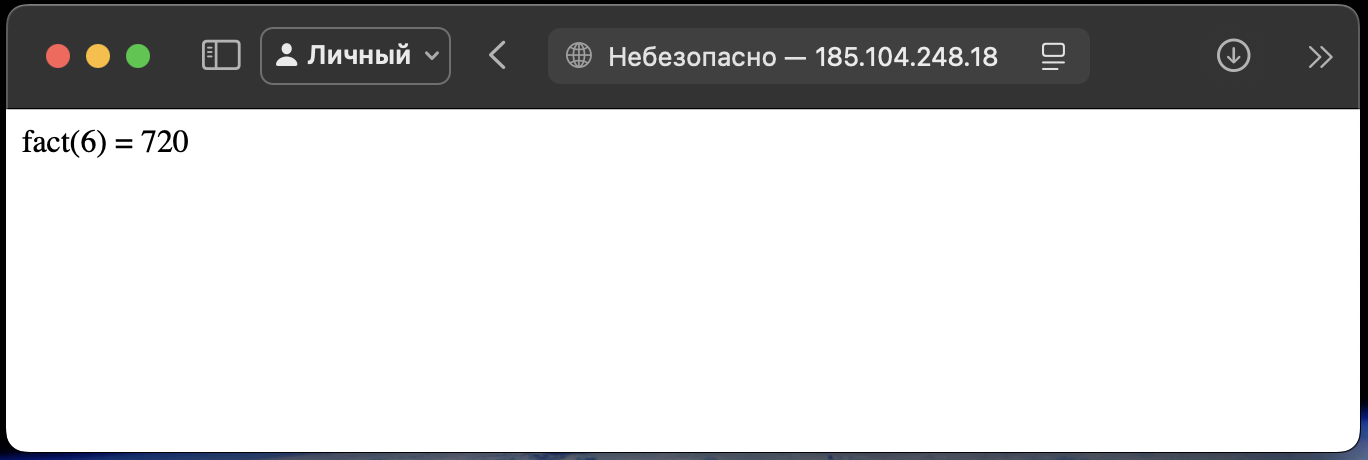
\includegraphics[width=0.8\textwidth]{images/photo5.png}
\caption{Результат работы веб-сервера}
\label{fig:photo2}
\end{figure}


\end{document}
